\chapter{Question1}
\section{问题概述}
%
%%对问题的直观描述
%
本问题要求改进已有的基于反射的智能体。这里需要考虑有多个幽灵的场景,默认情况下幽灵的行动是随机的,最后评分的依据首先是能够确保吃豆人不被幽灵击败并收集到所有的食物,
然后是分数尽可能地高。


%
%对项目已有代码的阅读和理解
%

%
%解决问题的思路和想法
%

\section{算法设计}
已有代码中实现的智能体选择下一个行为的唯一依据是下一个状态的得分。这不仅导致吃豆人收集所有
食物的效率大大降低——当四周没有食物时,很有可能会来回兜圈子,更重要的是,这几乎没有考虑幽灵对于吃豆人的影响——吃豆人可能会移动到幽灵的相邻位置,这导致
吃豆人暴露在被幽灵吃掉的风险之中,而这并不能体现在下一个状态的得分之中,因为这需要涉及到再下一个状态。

为此,应该充分利用幽灵的位置信息和剩余食物的位置信息,使得确保吃豆人不会被幽灵击败的前提下尽可能高效地收集所有食物。
为了保证吃豆人的安全,我们只需要确保下一个状态和幽灵的曼哈顿距离不小于等于1即可。

在确保没有被幽灵击败的前提下,我优先让吃豆人选择直接收集到食物的动作,如果没有,则以到最近的食物的曼哈顿距离的相反数为评估函数,即采用贪心的策略,让吃豆人缩短其到最近的食物的距离。
%
%用自己的语言描述解决问题所使用的算法的原理及功能,设计思路和算法流程图
%
\section{算法实现}
%
%在算法原理的基础上,结合代码,讲述算法的实现细节、核心函数、模块输入输出,数据结构定义等内容
%
\begin{lstlisting}[emph={[3]currentGameState,action},emphstyle={[3]\color{vscode_parametercolor}},emph={[4]GameState},emphstyle={[4]\color{vscode_classcolor}}]
def evaluationFunction(self, currentGameState: GameState, action):
    successorGameState = currentGameState.generatePacmanSuccessor(action)
    newPos = successorGameState.getPacmanPosition()
    newFood = successorGameState.getFood()
    newGhostStates = successorGameState.getGhostStates()
    newScaredTimes = [ghostState.scaredTimer for ghostState in newGhostStates]

    if action == 'Stop':  # 不允许停止
        return -float('inf')
    newGhostPos = [ghostState.configuration.pos for ghostState in newGhostStates]
    # 只有当不进入无敌状态时才要考虑和幽灵之间的距离
    if sum(newScaredTimes) == 0 and min([manhattanDistance(ghostPos, newPos) for ghostPos in newGhostPos]) <= 1:
        return -float('inf')
    foods = newFood.asList()
    # 没有食物,即该步使得游戏胜利
    if not foods:
        return float('inf')
    score = -min([manhattanDistance(food, newPos) for food in foods]) - 100000 * len(foods)
    return score
\end{lstlisting}
这里要求吃豆人永远不停止不动,但实际上,在特别极端的情况下,例如吃豆人位于角落,幽灵处于它的紧邻的对角位置时,静止不动以观察幽灵的下一步才是正确的。
实现时,我用惩罚项-100000*len(foods)来体现出收集食物的优先性。值得注意的是,如果某个动作使得吃豆人收集到了一个食物,那么在进入该函数时,
该食物已经从食物列表中移除出来了,如果仅仅依据到食物列表中各个食物的曼哈顿距离的最小值,是无法判断出这一步究竟是否能够收集到食物的。
\section{实验结果}
%
%对试验结果进行详细展示,对每个问题展示测试截图,对于测试用例进行描述说明,对于为通过测试的用例结合自己的算法进行分析,可以结合调试过程进行分析
%
我成功获得了本问题的所有分数。
\begin{figure}[htbp]
    \centering
    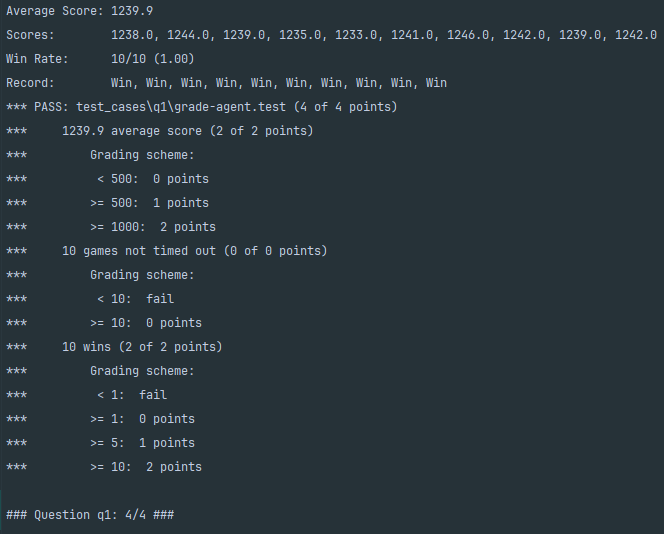
\includegraphics[scale = 0.7]{pic/q1.png}
    \caption{Question1实验结果}\label{q1}
\end{figure}

本问题的测试方式如图\ref{q1test}所示。该地图中没有墙壁,且只有一个随机移动的幽灵。通过该测试可以说明我所实现的算法能够指导吃豆人高效地收集所有的食物,
同时避免被幽灵击败。同时,我还额外对于有两个幽灵、有墙壁的中等迷宫场景进行了测试,如图\ref{q1ext},在连续两次测试中都成功收集所有的食物,结果如图\ref{q1extrst}所示。

\begin{figure}[htbp]
    \centering
    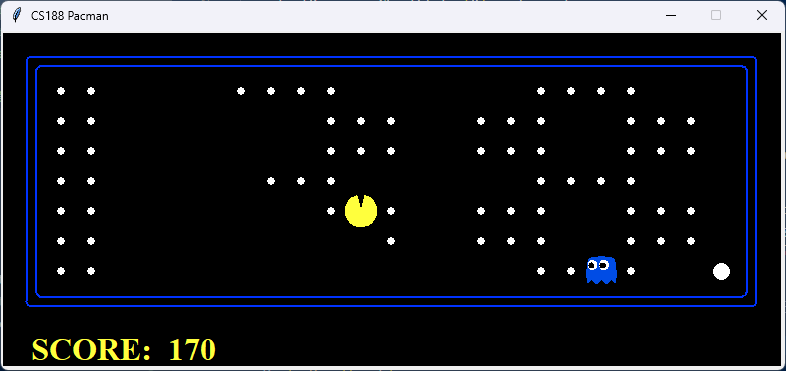
\includegraphics[scale = 0.5]{pic/q1test.png}
    \caption{Question1测试样例}\label{q1test}
\end{figure}
\begin{figure}[htbp]
    \centering
    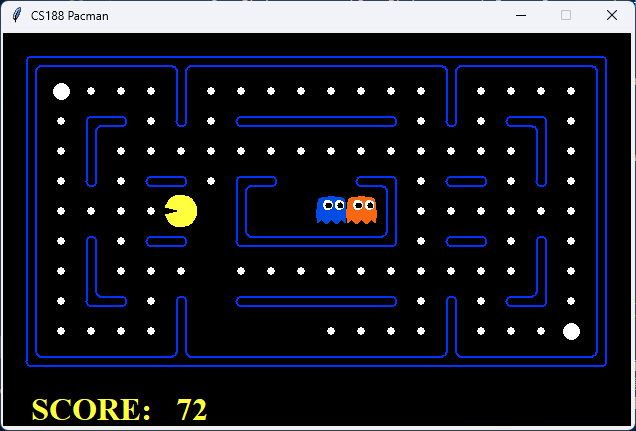
\includegraphics[scale = 0.5]{pic/q1ext.png}
    \caption{中等迷宫测试场景}\label{q1ext}
\end{figure}
\begin{figure}[htbp]
    \centering
    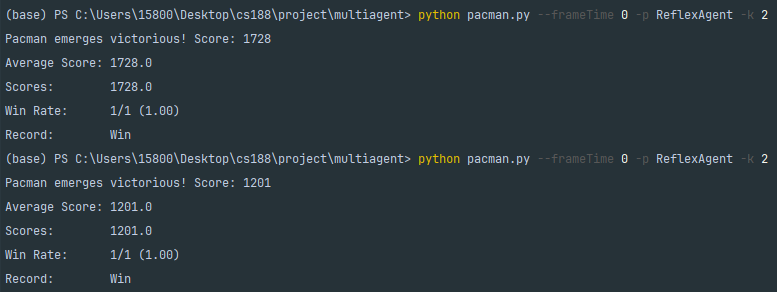
\includegraphics[scale = 0.8]{pic/q1extrst.png}
    \caption{中等迷宫测试结果}\label{q1extrst}
\end{figure}
%
%实验中遇到的问题及解决方案,收获和思考:对算法的理解、优缺点的评价、算法的适用场景
%
